\documentclass{article}
\usepackage{geometry}
\geometry{
	a4paper,
	%total={170mm,257mm},
	left=20mm,
	top=30mm,
}

\usepackage{fancyhdr}
\usepackage{tikz}
\usepackage{hyperref}
\usepackage{graphicx}
\usepackage{hyperref}
\usepackage{mdframed}
\usepackage{listings} % Include the listings package
\usepackage{xcolor}   % to define your own colors
\usepackage{subcaption}

\bibliographystyle{unsrt}
\bibliography{references}


\newmdenv[
linecolor=blue, % Color of the border line
backgroundcolor=gray!20, % Background color; "gray!20" means "20% gray"
frametitle=Note, % Title of the frame, delete this line if you don't want a title
skipabove=\baselineskip, % Space above the frame
skipbelow=\baselineskip, % Space below the frame
]{mynote}

% code-snippets:
% Define the color styles you wish to use in the document for the Python syntax highlighting
\lstdefinestyle{mystyle}{
	backgroundcolor=\color{white},   % choose the background color; you must add \usepackage{color} or \usepackage{xcolor}
	commentstyle=\color{green},
	keywordstyle=\color{blue},
	numberstyle=\tiny\color{gray},
	stringstyle=\color{red},
	basicstyle=\ttfamily\footnotesize,
	breakatwhitespace=false,         
	breaklines=true,                 
	captionpos=b,                    
	keepspaces=true,                 
	numbers=left,                    
	numbersep=5pt,                  
	showspaces=false,                
	showstringspaces=false,
	showtabs=false,                  
	tabsize=2
}
\definecolor{LightGray}{gray}{0.9}

\lstset{style=mystyle} % Apply your style globally to the document


\newcommand{\LVA}{Reverse Engineering}
\newcommand{\LVAKURZ}{REV3}
\newcommand{\SEMESTER}{WS 2023/2024}
\newcommand{\UELABEL}{UE 03}
\newcommand{\UETITLE}{Anti-Debugging}
\newcommand{\AUTHOR}{Jakob Mayr}


\title{\vspace{5cm} \LVA\ (\LVAKURZ)\\ \vspace{1cm} \textbf{\UELABEL\ -- \UETITLE\ -- Protokoll} \vspace{2.5cm}}
\author{\AUTHOR}
\date{\SEMESTER}

\begin{document}
	
	\pagestyle{fancy}
	
	\maketitle
	
	\tikz [remember picture, overlay] %
	\node [shift={(3.7cm,-4cm)}] at (current page.north west) %
	[anchor=north west] %
	{
\includegraphics{fhooe_logo.jpg}};
	
	\tikz [remember picture, overlay] %
	\node [shift={(10cm,-4.8cm)}] at (current page.north west) %
	[anchor=north west] %
	{
\includegraphics{si_logo.jpg}};
	
	%\tikz [remember picture, overlay] %
	%\node [shift={(7.2cm,-11.65cm)}] at (current page.north west) %
	%[anchor=north west] %
	%{\includegraphics[scale=0.12]{./img/star_wars_logo_no_background.png}};
	%
	%\pagebreak
	
	\fancyhf{}
	\fancyhead[L]{\LVA\ (\LVAKURZ)}
	\fancyhead[C]{\UELABEL}
	\fancyhead[R]{\SEMESTER}
	\fancyfoot[L]{Seite \thepage\ von \pageref{LastPage}}
	\fancyfoot[R]{\AUTHOR}
	
	\section*{Einleitung}
	...\\
	
	\pagebreak
	
	\section*{Implementierung}
	\subsection*{C}
	\begin{lstlisting}[language=c]
		#include <windows.h>
		
		/**
		* This function is a custom unhandled exception filter.
		*
		* @param ExceptionInfo A pointer to an EXCEPTION_POINTERS structure that
		*                      contains information about the exception.
		* @return A constant that determines how the exception is handled.
		*
		* The function displays a message box with the text "Infected" and
		* an icon indicating a warning. It's meant to be invoked when an
		* unhandled exception occurs. The function then returns a constant
		* indicating that the exception handler (EXCEPTION_EXECUTE_HANDLER)
		* should be executed.
		*/
		LONG WINAPI MyUnhandledExceptionFilter(struct _EXCEPTION_POINTERS* ExceptionInfo) {
			MessageBoxW(NULL, L"Infected", L"Infected", MB_ICONWARNING);
			
			//ExitProcess(0);
			
			return EXCEPTION_EXECUTE_HANDLER;
		}
		
		/**
		* The main entry point for the application.
		*
		* @return An integer indicating the success or failure of the program.
		*
		* The function first checks if a debugger is present using IsDebuggerPresent().
		* If a debugger is detected, it displays a message box with "Hello" and then
		* terminates. If no debugger is detected, it sets a custom unhandled
		* exception filter and then deliberately triggers a breakpoint exception
		* using DebugBreak(). If the breakpoint is unhandled, it will invoke the
		* custom unhandled exception filter. After handling the exception,
		* or if the breakpoint is handled by a debugger, it displays a "Hello" message
		* box and then exits.
		* 
		* NOTE: It might happen, that when executing this code on a system where a
		* debugger is just installed but not running, "DebugBreak()" or "INT 3" might
		* start the debugger automatically.
		*/
		int main() {
			
			if (IsDebuggerPresent()) {
				MessageBoxW(0, (LPCWSTR)L"Hello", (LPCWSTR)L"Hello", MB_OK);
				return 0;
			}
			SetUnhandledExceptionFilter(MyUnhandledExceptionFilter);
			DebugBreak();
			MessageBoxW(NULL, L"Hello", L"Hello", MB_OK);
			
			return 0;
		}
		
	\end{lstlisting}
	
	\pagebreak
	
	\subsection*{Assembler}
	\begin{lstlisting}[language={[x86masm]Assembler}]
.386
.model flat,stdcall
option casemap :none

include \masm32\include\windows.inc
include \masm32\include\kernel32.inc
include \masm32\include\user32.inc
includelib \masm32\lib\kernel32.lib
includelib \masm32\lib\user32.lib

.data
; Define strings to be used in the message boxes.
HelloWorld dw 'H','e','l','l','o',0
Infected dw 'I','n','f','e','c','t','e','d',0

.code
start:
	; Entry point of the program. Jumps to the 'begin' label.
	jmp begin

NoDebugger:
	; This section executes if no debugger is detected.
	; Displays a message box with the text "Infected" and a warning icon.
	push MB_ICONWARNING
	push offset Infected
	push offset Infected
	push 0
	call MessageBoxW
	jmp ExitProcessCall

begin:
	; Checks if a debugger is present.
	; Calls IsDebuggerPresent and examines the return value.
	call IsDebuggerPresent
	test eax, eax
	jnz DebuggerFound ; If EAX is non-zero, a debugger is detected, jump to DebuggerFound.
	
	; If no debugger is detected, set up an exception filter and trigger a breakpoint.
	invoke SetUnhandledExceptionFilter, NoDebugger
	int 3 ; Software breakpoint - triggers an exception if no debugger is present.
	; Continue to DebuggerFound if execution reaches here.
	jmp DebuggerFound

DebuggerFound:
	; This section executes if a debugger is detected.
	; Displays a message box with the text "Hello".
	push MB_OK
	push offset HelloWorld
	push offset HelloWorld
	push 0
	call MessageBoxW

ExitProcessCall:
	; Terminates the process.
	push 0
	call ExitProcess
	end start
	\end{lstlisting}
	
	\section*{Umgehung - Manuell}
	\subsection*{C}
	Um die Anti-debugging-Checks zu umgehen, gibt es mehrere Möglichkeiten.\\
	Für den Mechanismus "\texttt{IsDebuggerPresent()}" wurde der "JZ" nach dem Check zu einem "JNZ" geändert (umgekehrt ist dies natürlich auch möglich). Man siehe Addresse "\texttt{00401463}":\\
	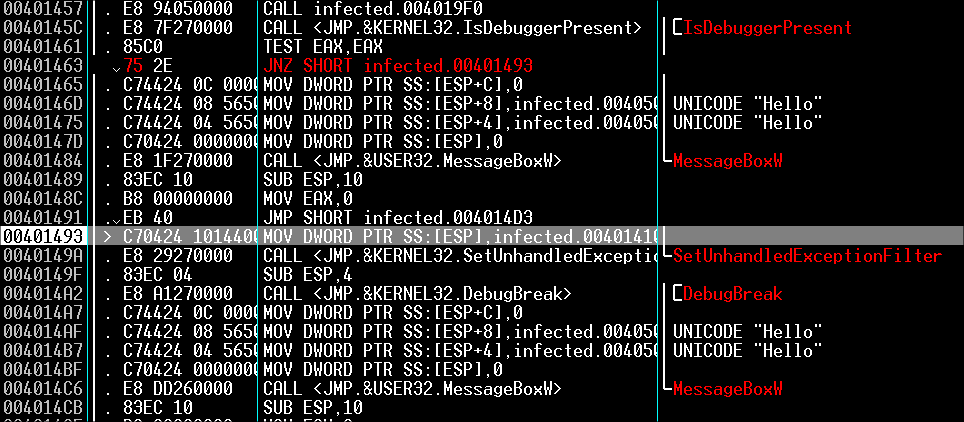
\includegraphics[width=0.7\linewidth]{"pictures/c - rev - isdebugged.png"}\\
	Für den Mechanismus "\texttt{Unhandled Exception}" muss ein wenig aufwendiger vorgegangen werden. Die Funktion "\texttt{SetUnhandledExceptionFilter}" setzt den Code welcher bei einer unabgearbeiteten (unhandled) Ausnahme (Exception) ausgeführt werden soll. Im folgenden Screenshot ist zu sehen, dass der Code an Adresse \texttt{00401410} ausgeführt werden soll:\\
	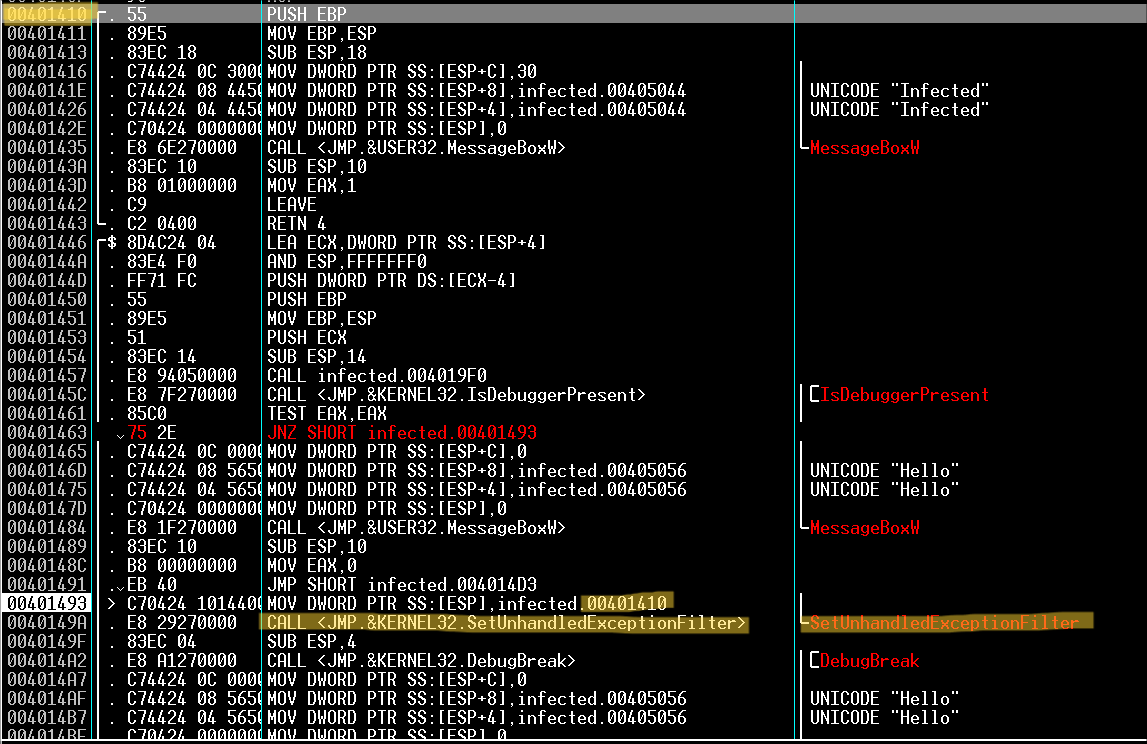
\includegraphics[width=0.7\linewidth]{"pictures/c - rev - unhandled exception.png"}\\
	Wird nun allerdings eine Ausnahme (Exception) ausgeführt, so arbeitet der Debugger diese anders ab und im Stack landet somit auch eine andere Rücksprungadresse. Diese kann allerdings während der Laufzeit geändert werden:\\
	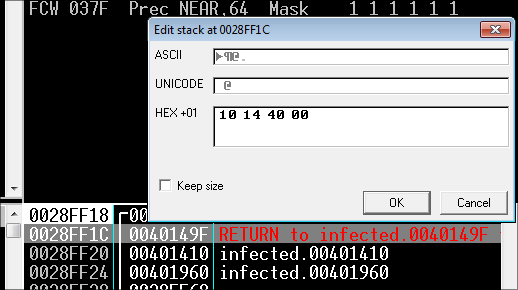
\includegraphics[width=0.7\linewidth]{"pictures/c - rev - unhandled exception - stack.png"}\\
	NOTE: Die Verwendung von "Ctrl+G" ist hierbei sehr hilfreich um Breakpoints an den einzelnen Funktionen zu setzen.\\
	
	\pagebreak
	
	\subsection*{Assembler}
	In Assembler könnte man ident vorgehen. Für den Mechanismus "\texttt{IsDebuggerPresent()}" wurde jedoch der "offset" des konditionalen Sprungs auf 0 gesetzt (Folge: macht nichts).\\
	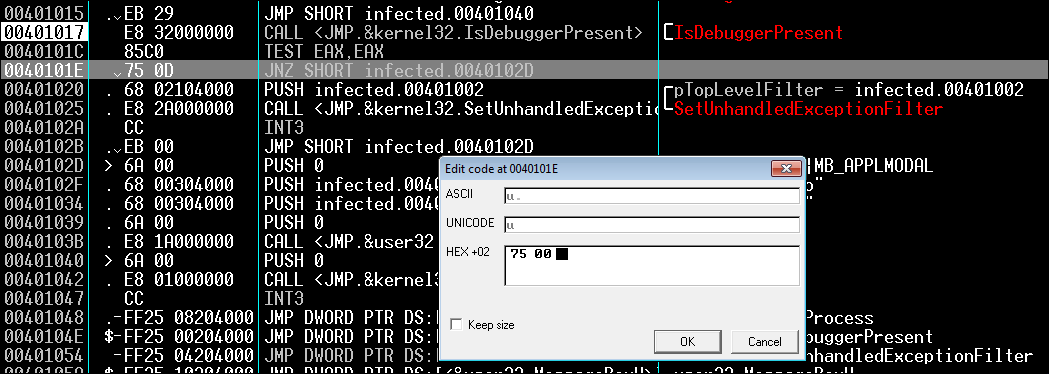
\includegraphics[width=0.7\linewidth]{"pictures/asm - rev - isdebugged.png"}\\
	Für den Mechanismus "\texttt{Unhandled Exception}" wurde wieder ein Breakpoint gesetzt und während der Laufzeit die Adresse für den auszuführenden Code geändert.\\
	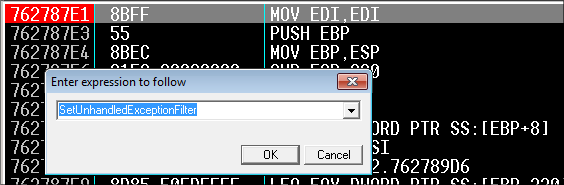
\includegraphics[width=0.7\linewidth]{"pictures/asm - rev - unhandled exception - breakpoint bei setunhandled exception.png"}\\
	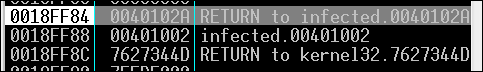
\includegraphics[width=0.7\linewidth]{"pictures/asm - rev - unhandled exception - stack.png"}\\
	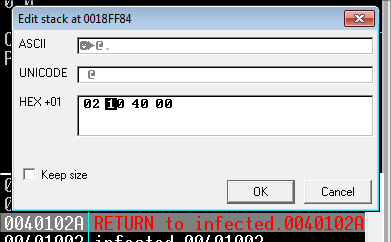
\includegraphics[width=0.7\linewidth]{"pictures/asm - rev - stack2.png"}\\
	
	\pagebreak
	
	\section{Plugins im Debugger}
	Nach Recherche im Internet wurde als Plugin die \texttt{PhantOm.dll} von "Roman Zaikin" t verwendet:\\
	\url{https://github.com/romanzaikin/OllyDbg-v1.10-With-Best-Plugins-And-Immunity-Debugger-theme-/blob/master/PhantOm.dll}\\
	Aktiviert man in OllyDbg das Plugin mit dem Profil "Optimal", so werden die Anti-Debugging Mechanismen simpel ausgehebelt.\\
	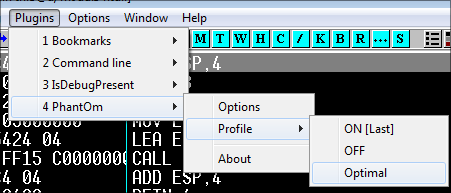
\includegraphics[width=0.7\linewidth]{"pictures/phantom.png"}\\
	Aktivierte Optionen des Plugins:\\
	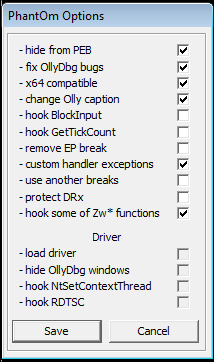
\includegraphics[width=0.2\linewidth]{"pictures/c - rev- plugin.png"}\\
	
	
	\label{LastPage}
	
\end{document}